%----------------------------------------------------------------
%
%  File    :  chapter6.tex
%
%  Authors : Michael Fuska, FH Campus Wien, Austria
%  Created : 13 Feb 2016
%
%  Changed :  
% 
%----------------------------------------------------------------


\chapter{Analyse und Ergebnisse}
\label{ch:Ergebnisse}

%------------------------------------------------------------------------------
%------------------------------ Analysen zur Frage 1

\section{Welche Faktoren sind für die Sicherheit und die Vertrauenswürdigkeit eines iOS Device ausschlaggebend?}
\label{sec:Frage1}

\begin{table}[htp!]
    \begin{center}
        \begin{tabular}{|p{30mm}|p{27mm}|p{12mm}|p{10mm}|p{18mm}|p{2cm}|p{15mm}|} \hline
            \textbf{iOS Device} & \textbf{Verkaufsstart} & \textbf{initial iOS} & \textbf{last iOS} & \textbf{Secure Enclave} & \textbf{Prozessor}  & \textbf{\#Tage JB} \\ \hline
            \textbf{iPhone} & 29.06.2007  & 1.0 & 3.1.3 & nA & Samsung SSL8900 & 11\\ \hline
            \textbf{iPhone 3G} & 11.07.2008 & 2.0 & 4.2.1 & nA & Samsung SSL8900 & 9\\ \hline
            \textbf{iPhone 3GS} & 19.06.2009 & 3.0 & 6.1.6 & nA & Samsung SSL8920 & 14\\ \hline
            \textbf{iPhone 4} & 01.08.2010 & 4.0 & 7.1.2 & nA & Apple A4 & 38 \\ \hline
            \textbf{iPhone 4s} & 20.01.2012 & 5.0 & 9.3.2 & nA & Apple A5 & 98 \\ \hline 
            \textbf{iPhone 5} & 21.09.2012 & 6.0 &  9.3.2 & nA & Apple A6 & 136 \\ \hline
            \textbf{iPhone 5c} & 22.12.2013 & 7.0 & 9.3.2 & nA & Apple A6 & 93 \\ \hline
            \textbf{iPhone 5s} & 22.12.2013 & 7.0 & 9.3.2 & A & Apple A7 & 93 \\ \hline
            \textbf{iPhone 6} & 19.09.2014 & 8.0 & 9.3.2 & A & Apple A8 & 33\\ \hline
            \textbf{iPhone 6 Plus} & 19.09.2014 & 8.0 & 9.3.2 &  A & Apple A8 & 33\\ \hline
            \textbf{iPhone 6s} & 25.09.2016 & 9.0 &  9.3.2 & A & Apple A9 & 19\\ \hline
            \textbf{iPhone 6s Plus} & 25.09.2016 & 9.0 & 9.3.2 &  A & Apple A9 & 19\\ \hline
            \textbf{iPhone SE} & 31.03.2016 & 9.0 &  9.3.2 & A & Apple A9 & nA\\ \hline  
        \end{tabular} 
        \caption{Auflistung iOS Device/ Verkaufsstart/ initial iOS/ last supported iOS / Prozessor/ \#Tage bis zum JB}
        \label{tab:iOSHW}
    \end{center}
\end{table}

In der Tabelle \ref{tab:iOSHW} werden alle iOS Devices aufgelistet und  in Abhängigkeit vom Verkaufszeitpunkt des Device, der initial installierten iOS Version und des Prozessor-Typs des iDevice gebracht. Zusätzlich wird in der Tabelle angeführt, ob diesem Device einen Koprozessor mit Secure Enclave zur Verfügung steht und wie lange die JB Community benötigte, um ein JB für dieses Device zu veröffentlichen. Diese Tabelle beinhaltet alle Daten die als Grundlage für alle weiteren Analysen in diesem Kapitel dienen.\par


%------------------------------------------------------------------------------
%------------------------------ 
\subsection{iOS Device}
\label{sec:Frage1iOSDevice} 

Die Tabelle \ref{tab:iOSHW} alleine gibt noch keinen Aufschluss über den Zusammenhang zwischen der Sicherheit des Systems und der verwendeten iOS Hardware. Da die Tabelle \ref{tab:iOSHW} keine Aussagen darüber zulässt, ob der Zeitraum bis zum Veröffentlichen des JB nur von der HW abhängt oder von der iOS Version die am Device installiert wurde. Aus diesem Grund müssen die Daten der beiden Tabellen (Tabelle: \ref{tab:iOSHW}, Tabelle: \ref{tab:iOSVersion}) korreliert werden. \par 
\begin{table}[htp!]
    \begin{center}
        \begin{tabular}{|l|l|l|} \hline
         \textbf{iOS Version} & \textbf{Veröffentilicht} & \textbf{\#Tage JB}\\ \hline    
        1.0 & 29.06.2007 & 11\\ \hline 
        2.0 & 11.07.2008	& 9\\ \hline 
        3.0 & 17.06.2009	& 2\\ \hline 
        4.0 & 21.06.2010 & 2\\ \hline 
        5.0 & 12.10.2011	& 1\\ \hline 
        6.0 & 19.09.2012	& 0\\ \hline 
        7.0 & 18.09.2013	& 95\\ \hline 
        7.1-7.1.2 & 29.05.2014 & 25\\ \hline 
        8.0 & 17.09.2014	& 35\\ \hline 
        8.1.1-8.4 & 17.11.2014	& 12\\ \hline 
        9.0 & 16.09.2015	& 28\\ \hline
       %  9.0.1 & 23.09.2015 & nA \\ \hline
       %  9.0.2 & 30.09.2015 & nA \\ \hline 
        9.1 & 21.10.2015	& 142\\ \hline 
       %  9.2 & 08.12,2015 & nA\\ \hline
       % 9.2.1 & 18.02.2016 & nA \\ \hline
       %  9.3 & 21.03,016 & nA\\ \hline 
       % 9.3.1 & 31.03.2016 & nA\\ \hline
       % 9.3.2 & 17.05.2016 & nA \\ \hline
        \end{tabular} 
        \caption{Auflistung iOS Version/ Veröffentlichungsdatum/ \# Tage bis zum JB}
        \label{tab:iOSVersion}
    \end{center}
\end{table}

Die Tabelle \ref{tab:iOSVersion} listet die iOS Version, das Veröffentlichungsdatum dieser iOS Version und die Anzahl an Tagen die benötigt wurden, um einen JB für diese iOS Version zu veröffentlichen auf.  \par 
\begin{figure}[htbp]
        \centering
                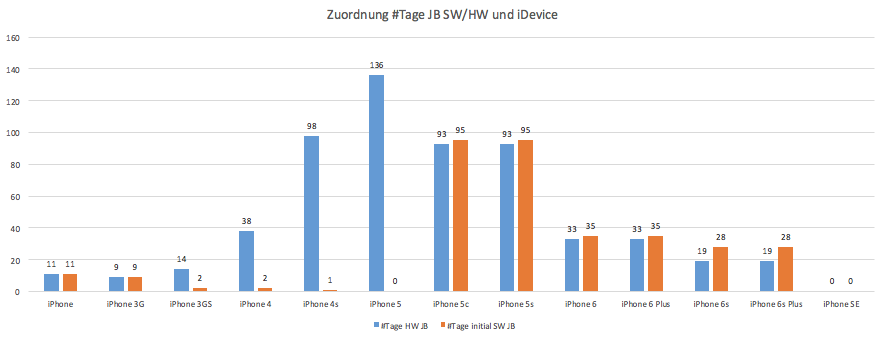
\includegraphics[scale=0.55]{Bilder/iDeviceJB-SW-HW.png}
         \caption{Vergleich der Anzahl der Tage eines JB für die Prozessoren und für der initialen iOS Version}
        \label{fig:VergleichJBProzessorSW}      
\end{figure}
Die Abbildung \ref{fig:VergleichJBProzessorSW} stellt die Verbindung zwischen dem Prozessoren des iDevices, der installierten iOS Version und der benötigten Tage für die Veröffentlichung eines JB her. Es kann gezeigt werden, dass alle Apple Prozessorarchitekturen einschliesslich des Apple A6 ein Sicherheitsgewinn für die iOS Produkte bedeutet haben. Dieser Schluss ist darauf begründet, dass die JBs für die selbe iOS Version auf älteren Apple Prozessorarchitekturen innerhalb von wenigen Tagen verfügbar war. \par 
Eine Veränderung ist in den Daten ist ab dem Apple A7 Prozessors sichtbar. Da zwischen dem veröffentlichen des JBs für die iOS Hardware und die iOS Version, nur mehr eine marginale Unterschied vorliegt.
\paragraph{Ergebnisse:} Dies lässt den Schluss zu, dass die Sicherheit und die Vertrauenswürdigkeit der iOS Produkte zum heutigen Zeitpunkt nur mehr von Apples mobilen Betriebssystem abhängt und nicht von der verwendeten iOS Hardware. 
% TODO
%64 BIT Architektur
%
%------------------------------------------------------------------------------
%------------------------------ 
\subsection{Secure Enclave}
\label{sec:Frage1SecureEnclave}
 
 Unter iOS gibt es die Möglichkeit verschiedene Passcode Konfigurationen vorzunehmen. Abhängig davon welche Prozessorgeneration verwendet wird, werden die Konfiguration und Daten des Passocdes in einer \textbf{Secure Enclave} oder im Flash Memory gespeichert. Neben der Anzahl der Stellen, kann auch konfiguriert werden, ob nur Zahlen oder auch alphanumerische Werte für einen Passcode verwendet werden.\par 
 Ein weiterer iOS Konfigurationsparameter ermöglicht es, das Device so zu konfigurieren, dass nach zehn falschen Passcode Eingaben alle Daten des Gerätes gelöscht werden. Die Anzahl der Fehlversuche wird bei iOS Devices ohne Secure Enclave in den Flash Memory geschrieben. Bei iOS Devices mit Secure Enclave werden diese Daten in der \textit{\glqq ARM Trust Zone\grqq{}} gespeichert und können somit nicht ohne weiters ausgelesen und überschrieben werden. 
 
% Die Secure Enclave des Koprozessor (siehe Tabelle: \ref{tab:iOSHW}) bringen einen massiven Sicherheitsgewinn für die iOS Produkte mit sich, da die  
 
 Im Fall \textit{\glqq FBI gegen Apple\grqq{}} wurde der Tatsache, dass das iOS Device keine Secure Enclave enthält, besonderer Bedeutung beigemessen. Das FBI beauftragte ein Unternehmen um das iPhone 5c des Attentäters zu entsperren. Die Abbildung: \ref{fig:iOSSecurityArchitekturiOS7} zeigt die iOS Sicherheitsarchitektur des iPhone 5c. Die Systemarchitektur dieses iOS Device beinhaltet keine Secure Enclave. \par 
\begin{description}
    \item[\parbox{\textwidth} { Der Sicherheitsforscher Zdziarski beschreibt in seinen Abhandlungen die plausiblen Varianten des FBI Hacks wie folgt}]~\par
    \begin{enumerate}
        \item \textit{\glqq .... based on all of this, is that an external forensics company, with hardware capabilities, is likely copying the NAND storage off the chip and frequently re-copying all or part of the chip’s contents back to the device in order to brute force the pin – and may or may not also be using older gear from iOS 8 techniques to do it. The two weeks the FBI has asked for are not to develop this technique (it’s most likely already been developed, if FBI is willing to vacate a hearing over it), but rather to demonstrate, and possibly sell, the technique to FBI by means of a field test on some demo units.\grqq{}} \cite{Hacking[4]}
        \item \textit{\glqq If the FBI did in fact use a software exploit, the question then becomes one of how viable it is on other platforms.\grqq{}} \cite{Hacking[4]}
    \end{enumerate}
\end{description} 

\paragraph{Ergebnisse:} Die Secure Enclave biete einen Sicherheitsgewinn für die iOS Produkte, aber der Fall \textit{\glqq FBI via Apple\grqq{}} lässt einige Fragen offen. Da das FBI, Apple die Sicherheitslücke nicht offenlegte gibt es nur Mutmaßungen, über den Hack der verwendet wurde, um das iPhone des Attentäters zu entsperren. \par 

Zdziarski beschreibt die möglichen Folgen dieses Hacks wie folgt: \textit{\glqq The moral of the story is that the exploit the FBI may have is dangerous in and of itself, regardless of whether it serves their specific purposes of brute forcing a device’s pin. Such an exploit has numerous uses within the intelligence community and poses a threat to not only the hundreds of millions of older devices out there, but if it can be ported to a 64-bit platform, every single one of us – either directly as a threat from the government, a nation state the exploit developer also sold it to, or another hacker who finds the same hole because FBI didn’t report the vulnerability to Apple. FBI has left us all potentially exposed by choosing to keep their technique secret.\grqq{}} \cite{Hacking[4]} \par 

Vor allem gibt es Vermutungen, dass der Hack des FBIs eine Möglichkeit bietet die Secure Enclave zu umgehen.


\newpage
%------------------------------------------------------------------------------
%------------------------------ 
\subsection{iOS Version}
\label{sec:Frage1iOSVersion} 

\begin{figure}[hp!]
        \centering
                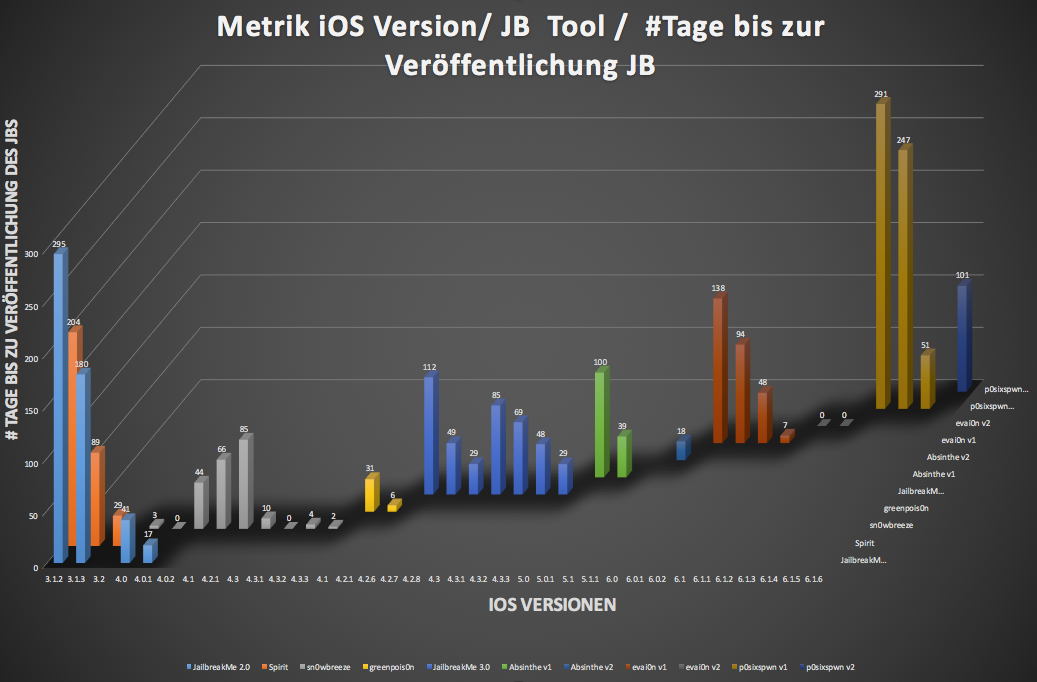
\includegraphics[scale=0.38]{Bilder/Frage1_1.png}
        \caption{iOS Version / JB Tools /\# Tage bis zum JB}
        \label{fig:AnalyseiOSJB1}        
\end{figure}

\begin{figure}[hp!]
        \centering
                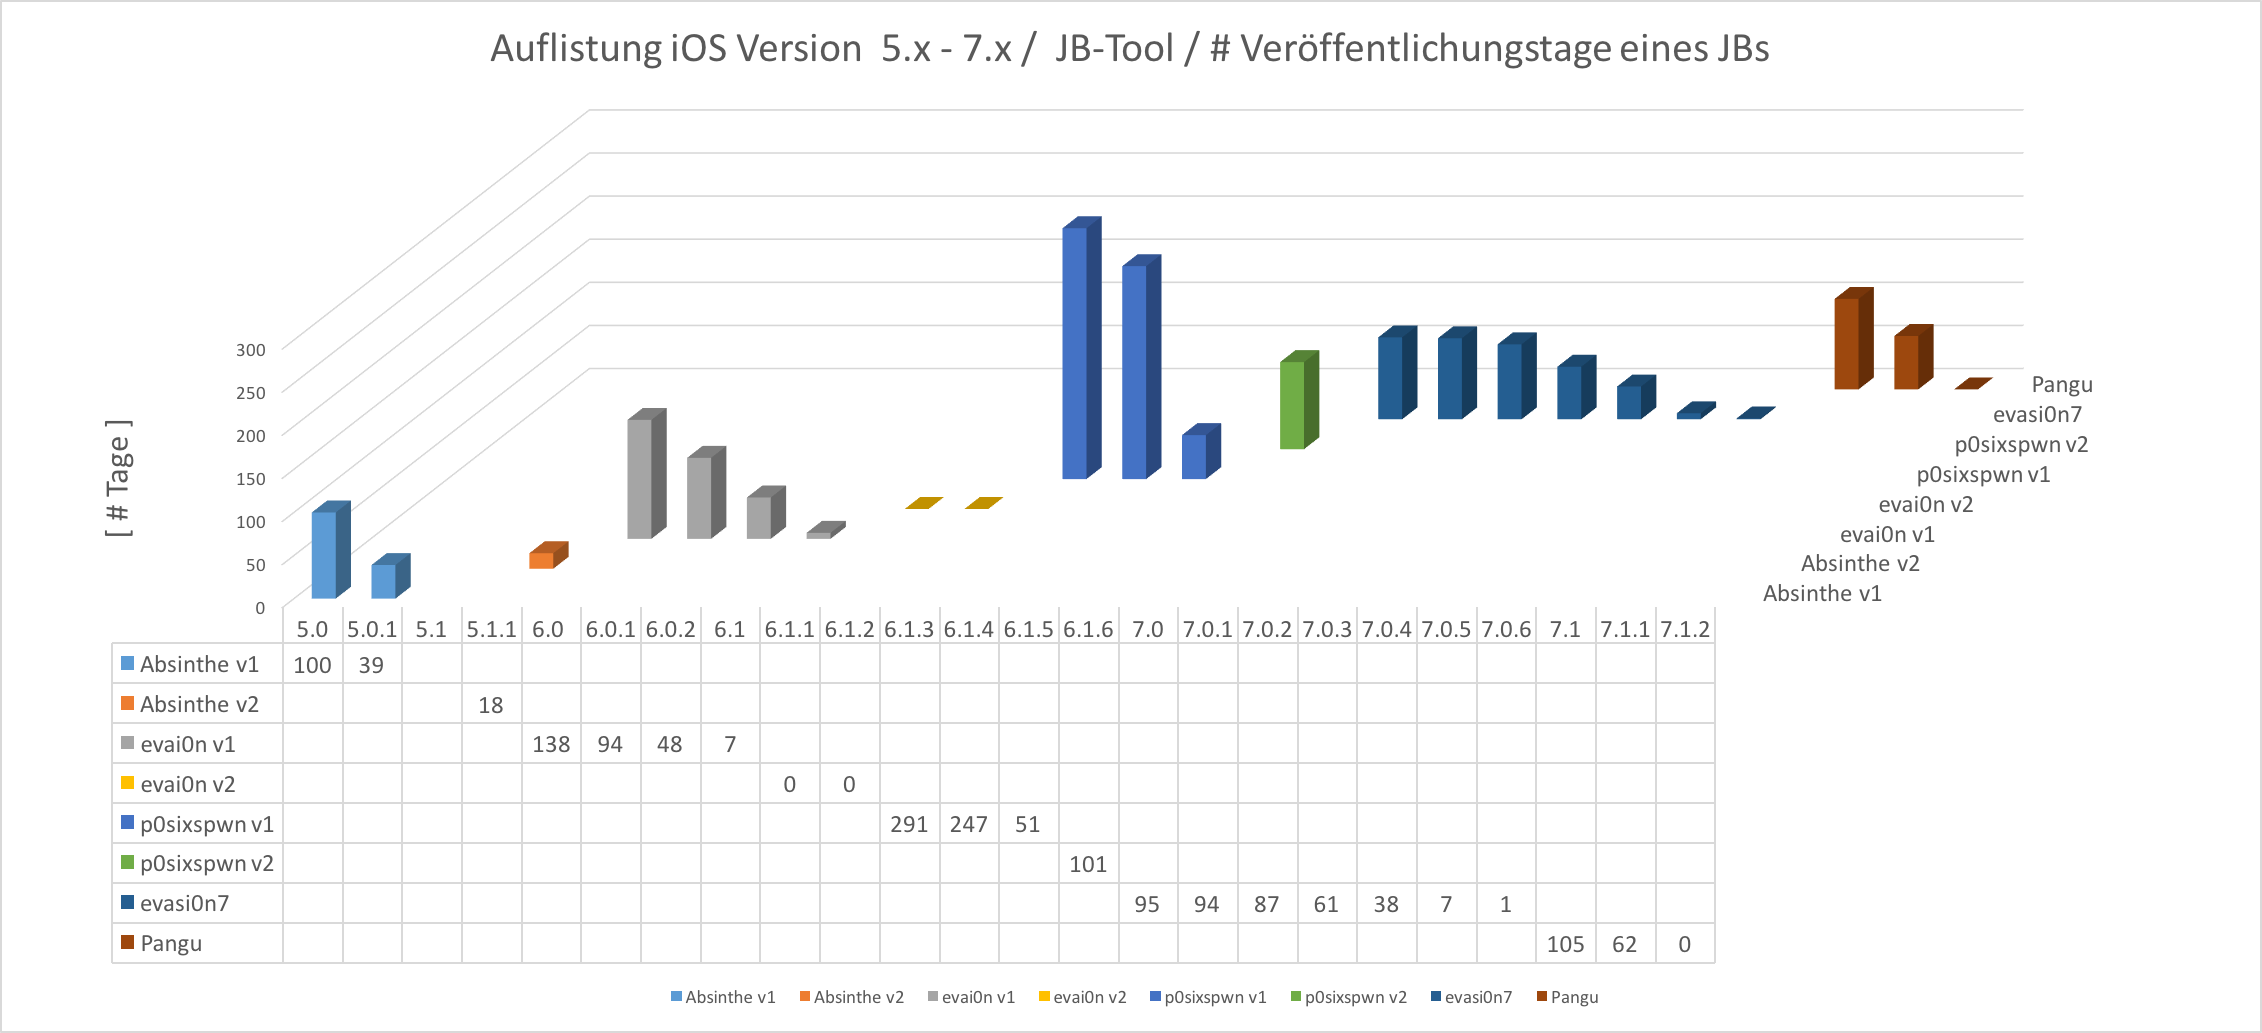
\includegraphics[scale=0.35]{Bilder/Frage1_2.png}
        \caption{iOS Version / JB Tools /\# Tage bis zum JB}
        \label{fig:AnalyseiOSJB2}
\end{figure}

Die Abbildungen \ref{fig:AnalyseiOSJB1} und \ref{fig:AnalyseiOSJB2} zeigen die bekanntesten und stabilsten untethered JBs, in Abhängigkeit mit der iOS Version und der Anzahl an Tagen die benötigt wurden, um für diese iOS Version ein Jailbreak bereitzustellen. \par 
\textbf{Die Graphiken zeigen,} dass ein JB immer nur für eine Serie von iOS Version funktioniert. In den meisten Fällen funktioniert der JB für die \textit{\glqq aktuelle\grqq{}} iOS Version und einigen iOS Versionen davor. Nach wenigen Wochen stellt Apple ein iOS Sicherheitsupdate zur Verfügung, welches das JB verhindert. Dieses Verhalt zieht sich durch alle betrachtet Metriken.  
%
%dass nach einem gelungen JB die Sicherheitsupdates von Apple einen kurzzeitigen Sicherheitsmehrwert mit sich bringen, aber innerhalb einiger Tage wurde ein neuer JB, des selben JB-Team veröffentlicht. Dies lässt darauf schliessen, dass die Sicherheitslücken nur teilweise geschlossen worden sind. Dieser Verhalten gilt  für alle iOS Versionen bis einschliesslich der iOS Version 9.x.\par  
%Ab der iOS Version 8.x ändert sich dieses Verhalten, da die JB Community jetzt länger für die JBs der nachfolgenden iOS minor Releases benötigt. \par 
%Markant ändern sich die Muster ab der iOS Version 9.x. Das JB für die Minor iOS Version 9.1 benötigte fast sechsmal länger, als das JB für die Major iOS Version 9.0 benötigte.\par



\begin{figure}[hp!]
        \centering
                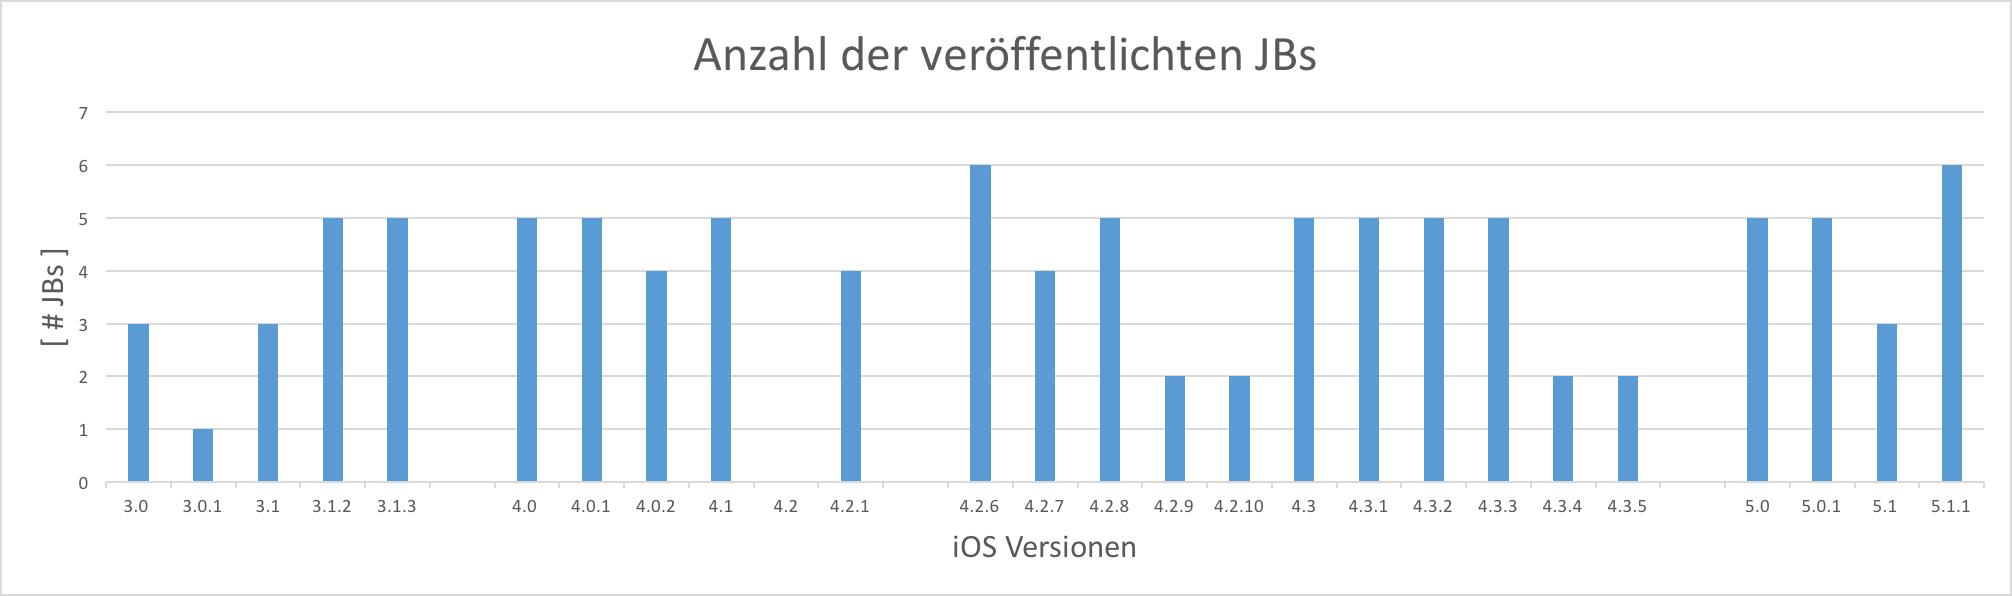
\includegraphics[scale=0.5]{Bilder/iOSJB1.png}
        \caption{Anzahl der veröffentlichten JBs pro iOS Version 3.x - 5.1.1}
        \label{fig:AnalyseAnzahliOSJB1}
\end{figure}

\textbf{Die Abbildungen \ref{fig:AnalyseAnzahliOSJB1} und \ref{fig:AnalyseAnzahliOSJB2} zeigen,} dass die Anzahl der veröffentlichten JB-Tools, ab der iOS Version 7.0 massiv rückgängig sind. Es wurden nur mehr ein oder zwei JB-Tools pro iOS Version der Öffentlichkeit zur Verfügung gestellt. 

\begin{figure}[hp!]
        \centering
                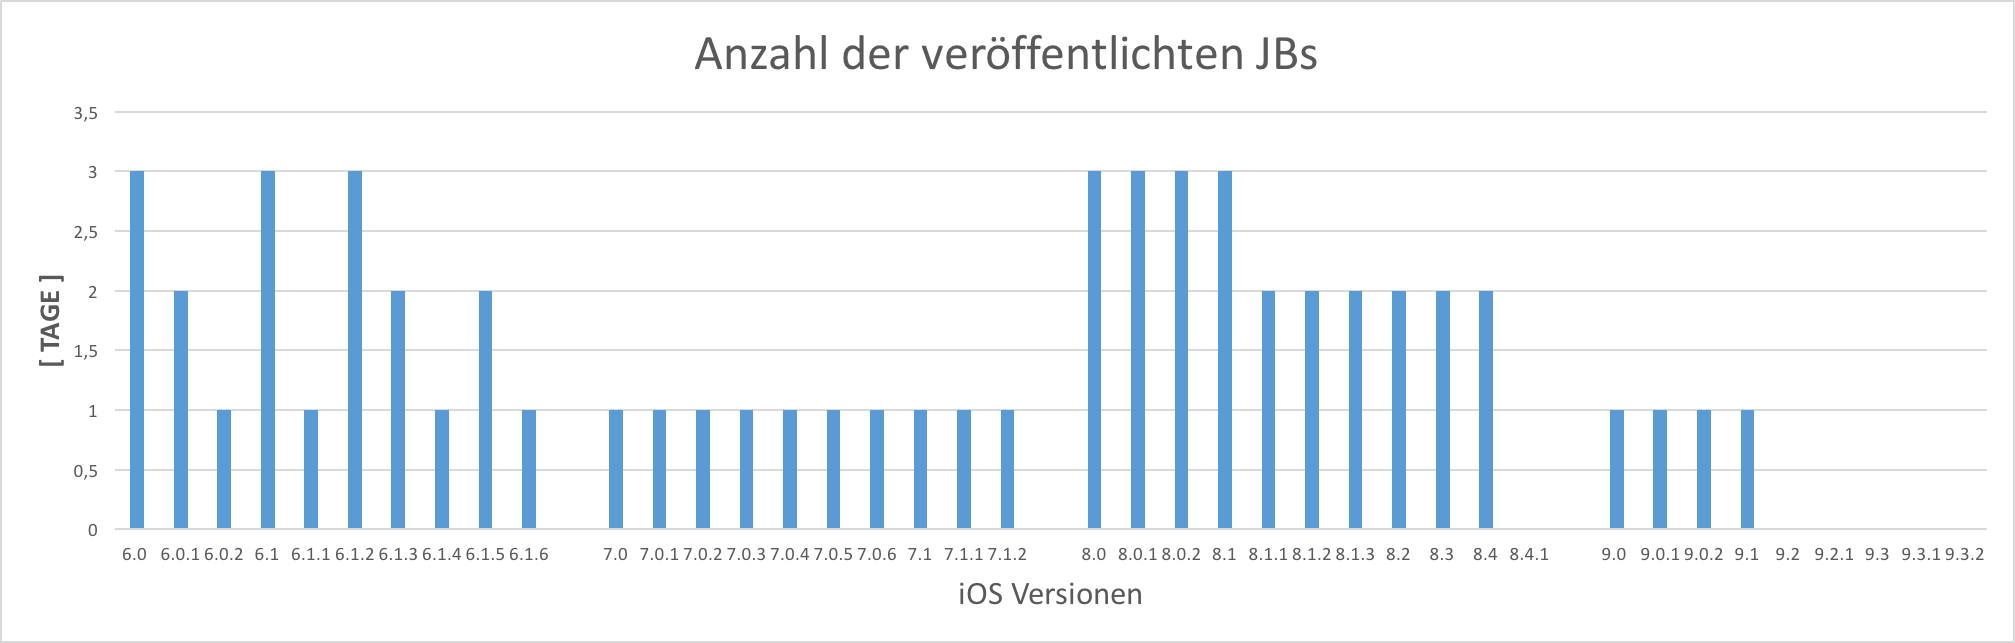
\includegraphics[scale=0.5]{Bilder/iOSJB2.png}
        \caption{Anzahl der veröffentlichten JBs pro iOS Version 6.x - 9.x.x}
        \label{fig:AnalyseAnzahliOSJB2}
\end{figure}


\paragraph{Ergebnisse:} Die aufbereitet Daten lassen den Schluss zu, dass die Sicherheit und die Vertrauenswürdigkeit der iOS Produkte mit steigender iOS Version zunimmt. Dieses Schluss ist darauf begründet, dass die Anzahl der Tage die benötigt wurden, um einen JB zur Verfügung zu stellen, eine steigende Tendenz aufweist. Der letzte untethered JB wurde Anfang Dezember 2015 veröffentlicht, seit diesem Zeitpunkt wurden sechs iOS Versionen veröffentlicht und es sind 243 Tage (per 18.07.2016) vergangen.\par 
Ein weiterer Anhaltspunkt für die Steigerung der Sicherheit ist, dass die Anzahl der Menschen die noch einen funktionsfähigen Jailbreak entwickeln können sinkt. 
\par 
Es muss darauf hingewissen werden, dass Apple seine Strategie im Bezug auf die JB Community geändert hat. In der Vergangenheit hat Apple versucht, gegen JBs gerichtlich vorzugehen, aber nur mit begrenzten Erfolg (\textit{\glqq Klage gegen George Hotz alias Geohot\grqq{}}). Apple hat vor einigen Jahren damit begonnen namhafte iOS Hacker anzustellen, unteranderem Comex  der Entwickler von \textit{\glqq JailbreakMe\grqq}. Dies bringt zwei Vorteile für Apple mit sich. Erstens, die Hacker kennen das mobile Betriebssystem und die Schwächen dieses, besser als viel interne Apple Entwickler.  Zweitens, die JB Community verliert ein aktives Mitglied. Als sehr viel schwerwiegender für die JB-Community einzustufen ist, dass durch den ehemaligen Hacker auch einige Zero-Day Bugs Apple gemeldet werden.\par
Seit dem Jahr 2015 ist der kommerzielle Aspekt in diesem Zusammenhang nicht ausser acht zu lassen. Angefangen mit dem Preisgeld welches auf ein JB der iOS Version 9.x ausgesetzt wurde, bis hin zu Premieren für Zero-Day Bugs. Dies hat meiner Meinung nach einen grossen Einfluss auf die Dauer der Veröffentlichung der JBs. Die markanten Ausreißer in den Metriken, ab der iOS Version 9.1 beruhen meiner Meinung nach auf dem kommerziellen Faktor. 

\newpage
%------------------------------------------------------------------------------
%------------------------------ 
\section{Welche Auswirkung haben die von Apple eingeführten Sicherheitsupdates auf die Sicherheit des Systems?}
\label{sec:Frage2}
%------------------------------------------------------------------------------
%------------------------------ 
%\subsection{iOS Sicherheitsmechanismen}
%\label{sec:Frage2SecMechanismen}
% 
%\begin{table}[htp!]
%    \begin{center}
%        \begin{tabular}{|l|l|l|l|} \hline
%            \textbf{Sicherheitsmechanismus} & \textbf{iOS 2.0} & \textbf{iOS 4.3} & \textbf{iOS 8.0} \\ \hline
%             Anzahl behobener Fehler & nA & 12 & 48\\ \hline
%             MAC & 8 & - & - \\ \hline
%             JIT & 8 & 85 & - \\ \hline
%             ASLR & - & 85 & - \\ \hline
%             verpflichtende Datenverschlüsselung & - & - & 35 \\ \hline
%             verpflichtende Datenverschlüsselung & - & - & 73\\ \hline
%        \end{tabular} 
%        \caption{Auflistung Sicherheitsmechanismus}
%        \label{tab:SecMechanismBugs}
%    \end{center}
%\end{table}

%------------------------------------------------------------------------------
%------------------------------ 
\subsection{iOS Sicherheitsupdates}
\label{sec:Frage2SecUpdate}

In diesem Kapitel wird auf die Wechselbeziehung zwischen der Sicherheit des iOS Device und den JBs, in Abhängigkeit der Hypothese H1 eingegangen. Im Detail wird die Historie einzelner JB-Tool betrachtet. 

\begin{table}[hp!]
    \begin{center}
        \begin{tabular}{| p{20mm} | p{12mm} | p{17mm} | p{12mm} | p{32mm} | p{22mm} | p{15mm} |} \hline
             \textbf{Datum iOS} & \textbf{iOS} & \textbf{\# Bugs} & \textbf{\# JB Bugs} & \textbf{JB Tool} & \textbf{JB Datum} & \textbf{\# Tage bis JB} \\ \hline 
            10.02.2011 & 4.2.6 &  - & -  & JailbreakMe 3.0 & 02.06.2011 & 112 \\ \hline
             09.03.2011 & 4.3 & 12 & 0 & JailbreakMe 3.0 &	02.06.2011 & 85 \\ \hline
             25.03.2011 & 4.3.1 &  - & - & JailbreakMe 3.0 & 02.06.2011 & 69 \\ \hline
            14.04.2011 & 4.2.7 &  4 & 0 & JailbreakMe 3.0 & 02.06.2011 & 49 \\ \hline
             15.04.2011 & 4.3.2 & 5 & 0 & JailbreakMe 3.0 & 02.06.2011 & 48 \\ \hline
             04.05.2011 & 4.2.8 &  - & - & JailbreakMe 3.0 & 02.06.2011 & 29 \\ \hline
            \textbf{04.05.2011} & \textbf{4.3.3} &  - & -  & \textbf{JailbreakMe 3.0} & \textbf{02.06.2011} & \textbf{29} \\ \hline
            15.07.2011 & 4.3.4 &  1 & 2	 & - & - & - \\ \hline
        \end{tabular} 
        \caption{Analyse JB-Tool JailbreakMe 3.0 \protect\footnotemark}         
        \label{tab:AnalyseJailbreakMe3.0}
    \end{center}
\end{table}
%iOS2011-2012
\footnotetext{\url{https://support.apple.com/de-de/HT204611}}
%\footnote{\label{foot:iOS2011-2012}{\url{https://support.apple.com/de-de/HT204611}}}

\paragraph{JailbreakMe 3.0} ist ein \textit{\glqq webbasierter Userland Exploit\grqq{}} und wurde am 02.06.2011 veröffentlicht. Dieser untethered Jailbreak wurde für die iOS Version 4.3.3 bereitgestellt. Es konnten aber mit diesem Exploit auch die iOS Version 4.2.6-4.3.3 (Siehe Tabelle: \ref{tab:AnalyseJailbreakMe3.0})  \textit{\glqq gejailbreaked\grqq{}} werden. 
Dieser Exploit nutzte einen Fehler im CoreGraphik Framework aus. Dieser ermöglicht es, im Zusammenhang mit dem Lesen eines PDFs, einen beliebigen Code auszuführen. Der IOMobileFrameBuffer hatte einen weiteren Softwarefehler, welcher es den JailbreakMe 3.0 Exploit ermöglichte, Systemprivilegien zu erhalten. Beide Bugs wurde in der iOS Version 4.3.4 \footnote{\label{foot:iOS4.3.4}{\url{https://support.apple.com/de-de/HT202272}}} geschlossen. Ab der iOS Version 4.3.4 ist dieser JB nicht mehr funktionsfähig.
 
\paragraph{Ergebnisse:} Interessant an den Daten der Tabelle \ref{tab:AnalyseJailbreakMe3.0} ist, dass in einem Zeitraum von 112 Tagen sechs iOS Sicherheitsupdates von Apple zur Verfügung gestellt wurden. In dieses sechs Updates wurden insgesamt 21 Bugs behoben. Das Schliessen dieser Sicherheitslücken hatte keine Auswirkung auf den später veröffentlichten JB. Dieses Verhalten zeigen sich in allen Analysen der JB-Tools. \par  
Am 15.07.2011 wurde das iOS Sicherheitsupdate 4.3.4 zum Download zur Verfügung gestellt. In diesem Update wurden insgesamt drei Sicherheitslücken von Apple geschlossen. JailbreakMe 3.0 verwendetet zwei von diesen Bugs und somit war der JB für alle weiteren iOS Version unterbunden. Dies zeigt, das Apple dieses JB-Tools \textit{\glqq reverse engineered\grqq{}} hat und gezielt Sicherheitsupdates zum Unterbinden dieser zur Verfügung stellt. Apple benötigte \textbf{43 Tage} um das Update bereitzustellen. Dadurch wird gezeigt, das die JBs einen direkten Einfluss auf die Sicherheit und Vertrauenswürdigkeit des iOS Systems haben, da Apple anhand der in der Analyse gefunden Bugs, Sicherheitsupdates zur Verfügung stellt. \par 

\begin{table}[hp!]
    \begin{center}
        \begin{tabular}{| p{15mm} | p{20mm} | p{17mm} | p{12mm} | p{20mm} | p{22mm} | p{15mm} |} \hline
            \textbf{iOS} & \textbf{Datum iOS} & \textbf{\# Bugs} & \textbf{\# JB Bugs} & \textbf{JB Tool} & \textbf{JB Datum} & \textbf{\# Tage bis JB} \\ \hline 
7.1 & 10.03.2014 & 20 & 4 & Pangu & 23.6.2014 & 105 \\ \hline
\textbf{7.1.1} & \textbf{22.04.2014} & \textbf{4} & \textbf{0} & \textbf{Pangu} & \textbf{23.6.2014} & \textbf{62} \\ \hline
7.1.2 & 30.06.2014 & 18 & 0 & Pangu & 23.6.2014 & -7 \\ \hline
 & & & & & & \\ \hline
8.0 & 17.09.2014 & 44 & 4 & Pangu8 & 22.10.2014 & 35 \\ \hline
8.0.1 & 24.09.2014 & - & - & Pangu8 & 22.10.2014 & 28 \\ \hline
8.0.2 & 25.09.2014 & - & - & Pangu8 & 22.10.2014 & 27 \\ \hline
\textbf{8.1} & \textbf{20.10.2014} & \textbf{5} & \textbf{0} & \textbf{Pangu8} & \textbf{22.10.2014} & \textbf{2} \\ \hline
8.1.1 & 17.11.2014 & 5 & 3 & - & - & - \\ \hline
 & & & & & & \\ \hline
9.0& 16.09.2015 & 71 & 1 & Pangu9 & 14.10.2015 & 28  \\ \hline
\textbf{9.0.1} & \textbf{23.09.2015} & \textbf{-} & \textbf{-} & \textbf{Pangu9} & \textbf{14.10.2015} & \textbf{21}\\ \hline
9.0.2 & 30.09.2015 & 1 & 0 & Pangu9 & 14.10.2015 & -14 \\ \hline
9.1(32 Bit) & 21.10.2015 & 25 & 2 & Pangu9 & 14.10.2015 & -  \\ \hline
		 & & & & & & \\ \hline				
\textbf{9.1(64 Bit)} & \textbf{21.10.2015} & \textbf{25} & \textbf{2} & \textbf{Pangu9} & \textbf{11.3.2016} & \textbf{142}  \\ \hline
9.2 & 08.12.2015	 & 27 & 3 & - & - & - \\ \hline		
     \end{tabular} 
        \caption{Analyse JB-Tool Pangu \protect\footnotemark}
        \label{tab:AnalysePangu}
    \end{center}
\end{table}
%{\label{foot:iOS2015-2016}
%\footnote{\url{https://support.apple.com/de-de/HT201222}}
\footnotetext{\url{https://support.apple.com/de-de/HT201222}}

\paragraph{Das JB-Team Pangu} veröffentlicht in den letzten zwei Jahren JBs für drei Major iOS Versionen. Bevor das Team Pangu ihren ersten JB veröffentlichte, nahmen die Member des Teams an einem iOS Exploitation Trainings von von Stefan Essers teil \footnote{\url{https://www.sektioneins.de/en/trainings/iosexploitation.html}}. Zu Kontroversen führte dieser JB, da dieser auf den im Training vorgeführten Kernel Exploits beruhte.\par
Bis zum heutigen Datum (18.07.2016) wurden vom Pangu Team vier unterschiedliche JB Version veröffentlicht. Mit diesen vier JBs können zwölf iOS Versionen \textit{\glqq gejailbreaked\grqq{}} werden (siehe Tabelle: \ref{tab:AnalysePangu}).

Die Tabelle \ref{tab:AnalysePangu} zeigt, das selbe Muster, wie in den zuvor analysierten JB-Tool JailbreakMe 3.0. Mit einer Ausnahme, das nächste iOS Sicherheitsupdate 9.0.2 verhinderte nicht den JB der vierzehn Tage zuvor veröffentlicht wurde. \par 
Pangu Team veröffentlichte als erstes JB-Team einen JB für die neue 64 Bit Architektur veröffentlicht. 

\paragraph{Ergebnisse:}  Die iOS Version 7.1.2 ist das letzte Sicherheitsupdate für das iPhone 4. Für dieses Device, ist somit das letzte verfügbare Update, als nicht sicher einzustufen. \par 
Interessant ist auch, dass das iOS Sicherheitsupdate 8.1.1 drei Softwarefehler behebt, die vom JB-Tool Pangu8 verwendet wurden. Nach \textbf{26 Tage} wurde die Sicherheitslücken geschlossen, die den JB Pangu8 ermöglichten. Das iOS Sicherheitsupdate 8.1.1 hatte aber nur eine geringen Einfluss auf das JB-Tool TaiG. Dies zeigt deutlich, dass Apple gezielt Bugs von einzelnen JB-Tool schliesst. 

Apple schloss in der iOS Version 9.0 zweiundsiebzig Sicherheitslücken und das JB-Team Pangu benötigte 28 Tage um diese Version zu \textit{\glqq jailbreaken\grqq{}}. Die iOS Version 9.2 beendete nach \textbf{55 Tagen} die Funktionsfähigkeit des JB-Tools Pangu9 . Daraus kann geschlossen werden, dass die Anzahl an geschlossenen Sicherheitsfehlern keinen direkten Einfluss auf den JB haben.

\begin{table}[htp!]
    \begin{center}
        \begin{tabular}{| p{10mm} | p{22mm} | p{17mm} | p{12mm} | p{18mm} | p{22mm} | p{15mm} |} \hline
            \textbf{iOS} & \textbf{Datum iOS} & \textbf{\# Bugs} & \textbf{\# JB Bugs} & \textbf{JB Tool} & \textbf{JB Datum} & \textbf{\# Tage bis JB} \\ \hline 
8.0 & 17.09.2014 & 44 & 4 & TaiG & 29.11.2014 & 73  \\ \hline
8.0.1 & 24.09.2014	& - & - & TaiG & 29.11.2014 & 66 \\ \hline
8.0.2 & 25.09.2014 & - & -  & TaiG & 29.11.2014 & 65  \\ \hline
8.1 & 20.10.2014 & 5 & 0 & TaiG & 29.11.2014 & 40  \\ \hline
\textbf{8.1.1} & \textbf{17.11.2014} & \textbf{5} & \textbf{3} & \textbf{TaiG} & \textbf{29.11.2014} & \textbf{12}  \\ \hline
 & & & & & & \\ \hline						
\textbf{8.1.2} & \textbf{09.12.2014} & \textbf{1} & \textbf{0} & \textbf{TaiG v2} & \textbf{08.03.2015} & \textbf{89}  \\ \hline
	 & & & & & & \\ \hline						
8.1.3 & 27.01.2015 & 16 & 5 & TaiG v3 & 23.06.2015 & 147  \\ \hline
8.2  & 09.03.2015 & 5 & 1 & TaiG v3 & 23.06.2015 & 106 \\ \hline
\textbf{8.3} &  \textbf{08.04.2015} & \textbf{40} & \textbf{1} & \textbf{TaiG v3} & \textbf{23.06.2015} & \textbf{103}  \\ \hline
		 & & & & & & \\ \hline					
\textbf{8.4} &  \textbf{30.06.2015} & \textbf{25} & \textbf{0} & \textbf{TaiG v4} & \textbf{01.07.2015} & \textbf{1}  \\ \hline
8.4.1 & 13.08.2015 & 35 & 9 & - & - & -   \\ \hline
        \end{tabular} 
        \caption{Analyse JB-Tool TaiG \protect\footnotemark}
        \label{tab:AnalyseTaig}
    \end{center}
\end{table}

%{\label{foot:iOS2014}
%\footnote{\url{https://support.apple.com/de-de/HT205762}
\footnotetext{\url{https://support.apple.com/de-de/HT205762}}

\paragraph{TaiG} zeigt wie kein anderes JB-Tool wie sehr Apple und die JB-Community Katz und Maus spielen  (siehe Tabelle: \ref{tab:AnalyseTaig}). Apple antwortete innerhalb weniger Tage mit einem Update, welches das JB schliesst. Das JB-Team TaiG veröffentlicht für jedes iOS Sicherheitsupdate ein neues JB. Bis am Ende Apple das iOS Sicherheitsupdate 8.4.1 veröffentlicht. In diesem Update werden acht Softwarefehler geschlossen, auf denen der TaiG JB aufbaute. 
 
Das iOS Sicherheitsupdate 8.1.2 wurde \textbf{zehn Tage} nach dem JB-Tool TaiG veröffentlich und behob die Sicherheitslücken der iOS Version 8.1.1. Dadurch funktionierte der TaiG JB in der iOS Version 8.1.2 nicht mehr.

Das JB-Tool TaiG v2 war schon bei seiner Veröffentlichung \textbf{nicht mehr obsolet}, da das iOS Sicherheitsupdate 8.1.3 schon zuvor veröffentlicht wurde. In diesem wurden fünf Sicherheitslücken geschlossen, auf denen das JB-Tool TaiG v2 aufbaute.
Die Sicherheitslücken die das JB-Tool TaiG v3 verwendet wurden teilweise nach \textbf{sieben Tagen} im iOS Sicherheitsupdate 8.4 geschlossen. In diesem iOS Sicherheitsupdate wurden 25 Bugs geschlossen, aber schon nach einem Tag wurde das JB-Tool TaiG v4 veröffentlicht. Die iOS Version 8.4.1 beendete nach \textbf{43 Tagen} die Funktionsfähigkeit des JB TaiG v4.

\begin{table}[htp!]
    \begin{center}
        \begin{tabular}{| p{10mm} | p{40mm} | p{17mm} |} \hline
            \textbf{iOS} & \textbf{JB-Tool} & \textbf{\# Tage} \\ \hline 
                4.3.4 & JailbreakMe 3.0 & 43 \\ \hline
                8.1.1 & Pangu8 & 26 \\ \hline
                9.2 & Pangu9 & 55 \\ \hline
                8.1.2 & TaiG & 10  \\ \hline
                 8.1.3 & TaiG v2 & - \\ \hline
                  8.4 & TaiG v3 & 7  \\ \hline
                  8.4.1 & TaiG v4 & 43  \\ \hline
        \end{tabular} 
        \caption{Apple Reaktionszeit auf ein JB}
        \label{tab:AppleReaktionszeit}
    \end{center}
\end{table}

\begin{figure}[hp!]
        \centering
                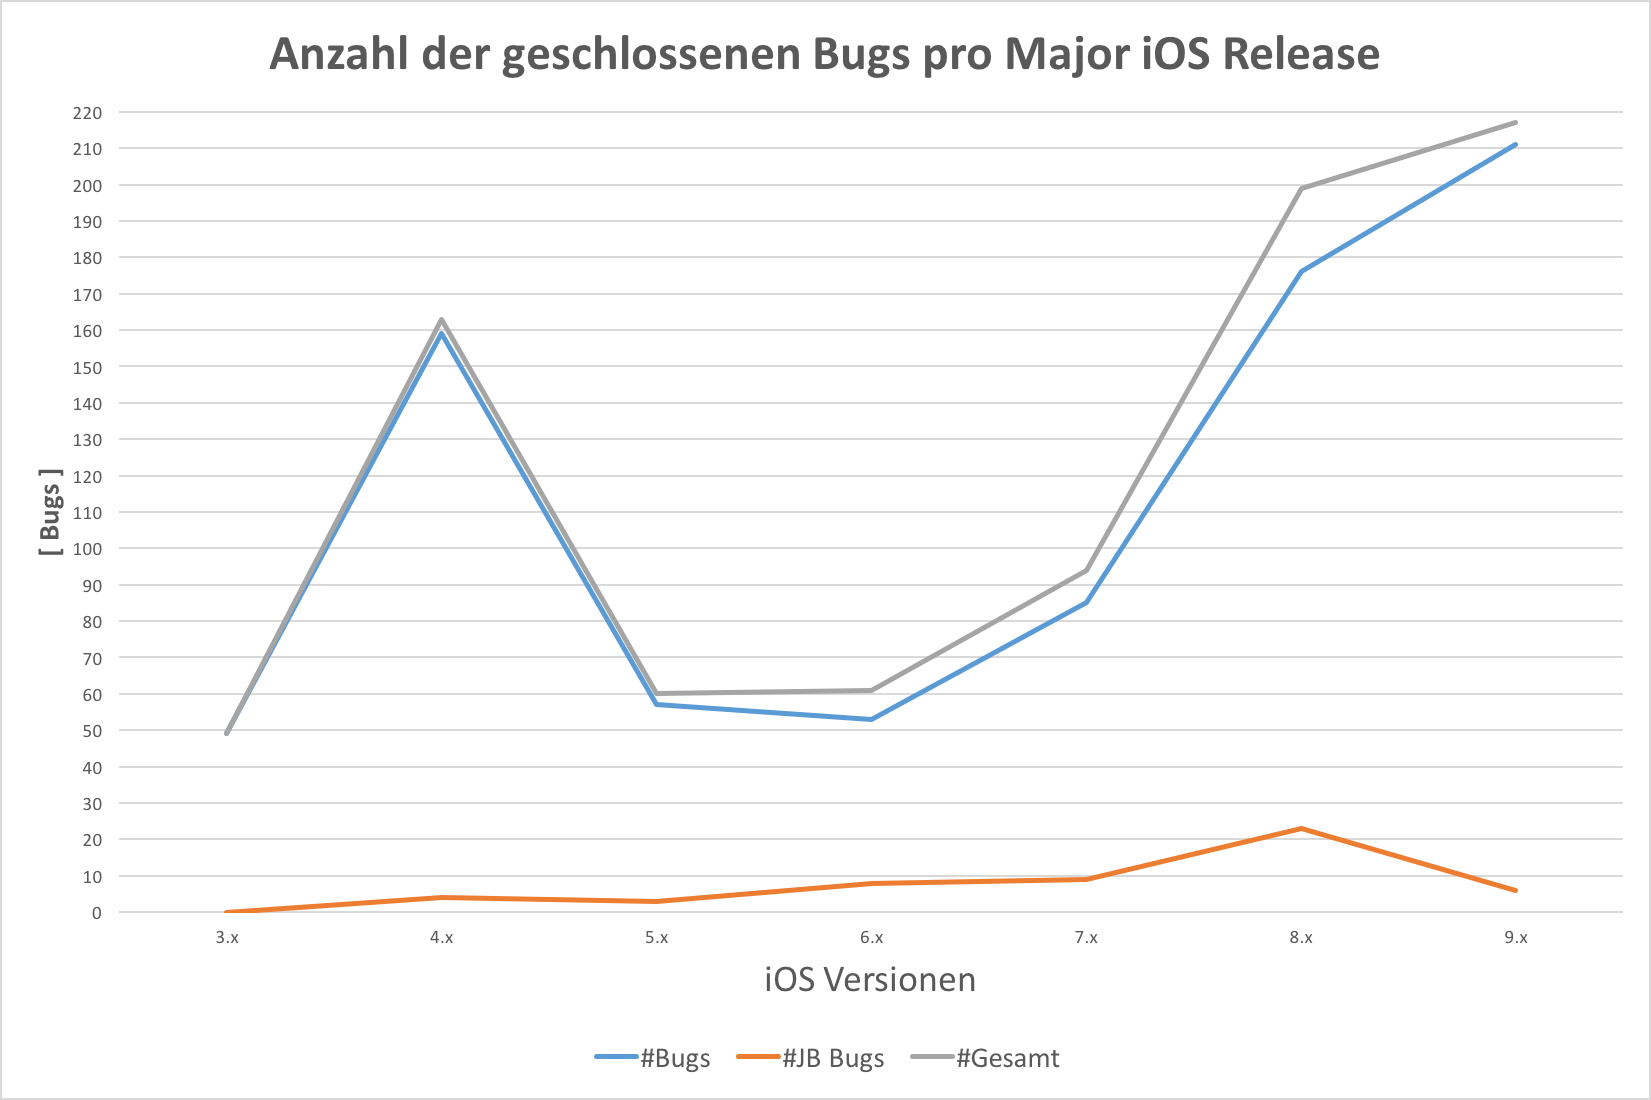
\includegraphics[scale=0.45]{Bilder/SecUpdateMajor.png}
        \caption{Anzahl Bugs pro iOS Major Release}
        \label{fig:SecUpdateMajor}
\end{figure}
%------------------------------------------------------------------------------
%------------------------------ 
\section{Analyse der Hypothese H1}
\label{sec:AnalyseHypo}

Die Daten zeigen, dass die Hypothese H1 (siehe Kapitel: \ref{sec:GQMHypothese}) nicht bestätigt werden kann. Die Anzahl an Tagen die für ein JB benötigt wird, hängen von zu vielen anderen Faktoren ab. 

\begin{description}
    \item[\parbox{\textwidth} {Neben der Sicherheit der iOS Versionen haben folgende Faktoren einen Einfluss auf die Veröffentlichungsdauer eines JBs}]~\par
    \begin{enumerate}
       \item die mangelnde Kontinuität der JB-Teams, 
       \item der kommerzielle Faktor, 
       \item  und das die JB Community ihre JBs zurück halten, wenn Apple bekannt gibt, dass eine neue Major Release veröffentlicht wird.   
   \end{enumerate}
\end{description} 
Diese Faktoren können nicht aus den Daten, auf denen diese Arbeit aufbaut, extrahiert werden und deshalb kann die Hypothese nicht bestätigt werden.



    